\chapter{設計}
\label{chap:design}
本章では設計について述べる。

\newpage
\section{Rive日本語入力システム}
Rive日本語入力システムは以下のものによって構成されている
\begin{itemize}
  \item Rive Client
  \item Rive Server
  \item Rive Analytics
  \item Rive Btachprocessing
  \item Rive Webservice
\end{itemize}
これらのシステムがお互いに作用することで
Rive日本語入力システムが実現されている。
\begin{figure}[htbp]
  \begin{center}
    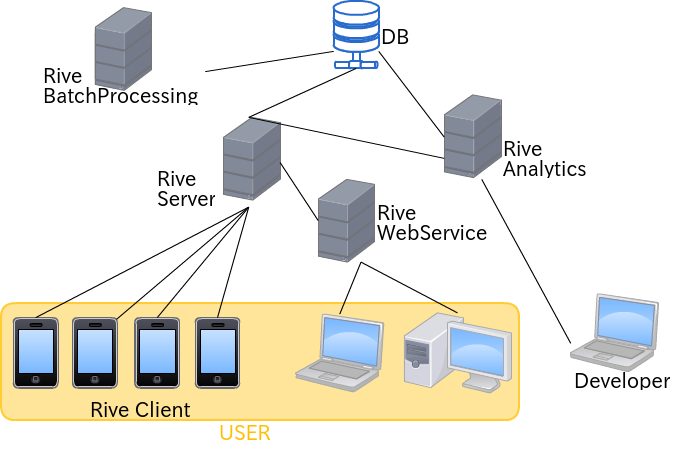
\includegraphics[width=12cm,bb=0 0 540 448]{images/systemstructure.png}
  \end{center}
  \caption{システム全体構成図}
  \label{fig:systemstructure}
\end{figure}

\section{Rive Client}
モバイルデバイスで利用可能なIMEアプリケーション本体。
ユーザーは基本的にこのシステムのみ使用する。
始めにRive Serverにコンテキストデータを送る。
その後帰ってきたデータを推薦候補単語として表示する。

\section{Rive Server}
Rive日本語入力における適切な候補単語を推測するサーバーの総称。
Rive Clientから受け取ったデータを解析し、
適切な推薦を行う。
また入力後のデータをRive Analyticsに送信する。

\section{Rive Analytics}
文字入力のデータを受け取り解析することで開発者の手助けをするシステム。

\section{Rive Batchprocessing}
定期的に処理を行うシステムの総称。

\section{Rive Webservice}
システムを試用するためのWEBページとして実装。
またRive日本語入力の紹介も兼ねている。

\section{システム間通信}
Rive ClientとRive Server間の通信はWebsocket、
その他システム間はhttpによって実現した。
